\section{実装試験}
\label{tag:experiment}
本研究ではLTIを用いることで実際に複数のLMSから、独立したWebアプリケーションであるネットワーク自己学習機能を同じように学習支援ツールとして呼び出すことができるのかを確認するために、LTIに準拠したLMSであるMoodle、Canvasを用いての実装実験を行った。\\

%\subsection{LTI使用方法}
LMS上でTool Providerを使用するには、各LMS上で外部ツールの設定を変更する必要がある。例として、moodleでの使用方法を説明する。\\
moodleでは外部ツール設定より、ツール名、ツールURL、コンシューマキー、秘密鍵の設定。これらの設定を得て、moodleからTool Providerを利用することが可能となる。\\
 
%\begin{figure}[htbp]
%  \begin{center}
%    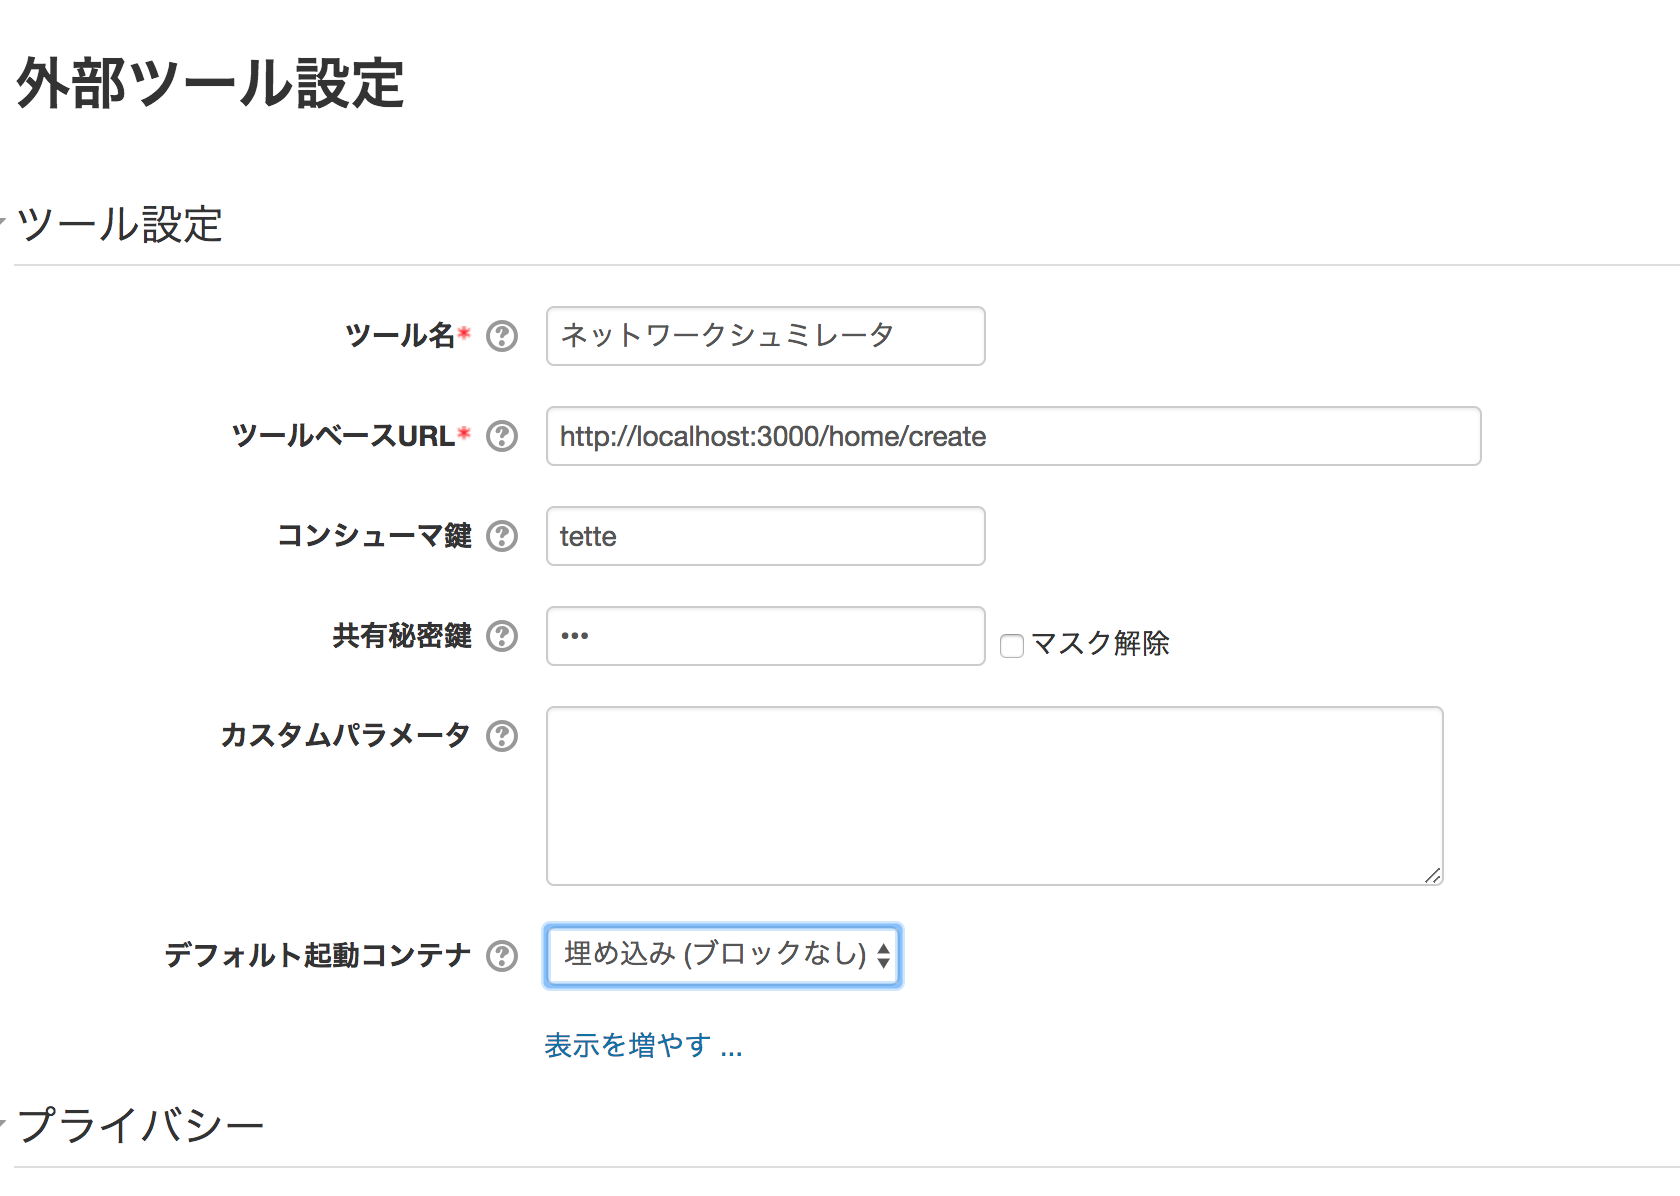
\includegraphics[scale=0.3]{img/moodleSet.png}
%    \caption{moodle 外部ツール設定画面}
%    \label{fig:moodle config}
%  \end{center}
%\end{figure}

%\subsection{成績反映}
Moodleにおいて、実際に成績反映できるかどうかの実験を行った。
%Moodleに置いて、成績の反映ができていることを確認した。
結果を図\ref{fig:moodle score}に示す。
\begin{figure}[htbp]
  \begin{center}
    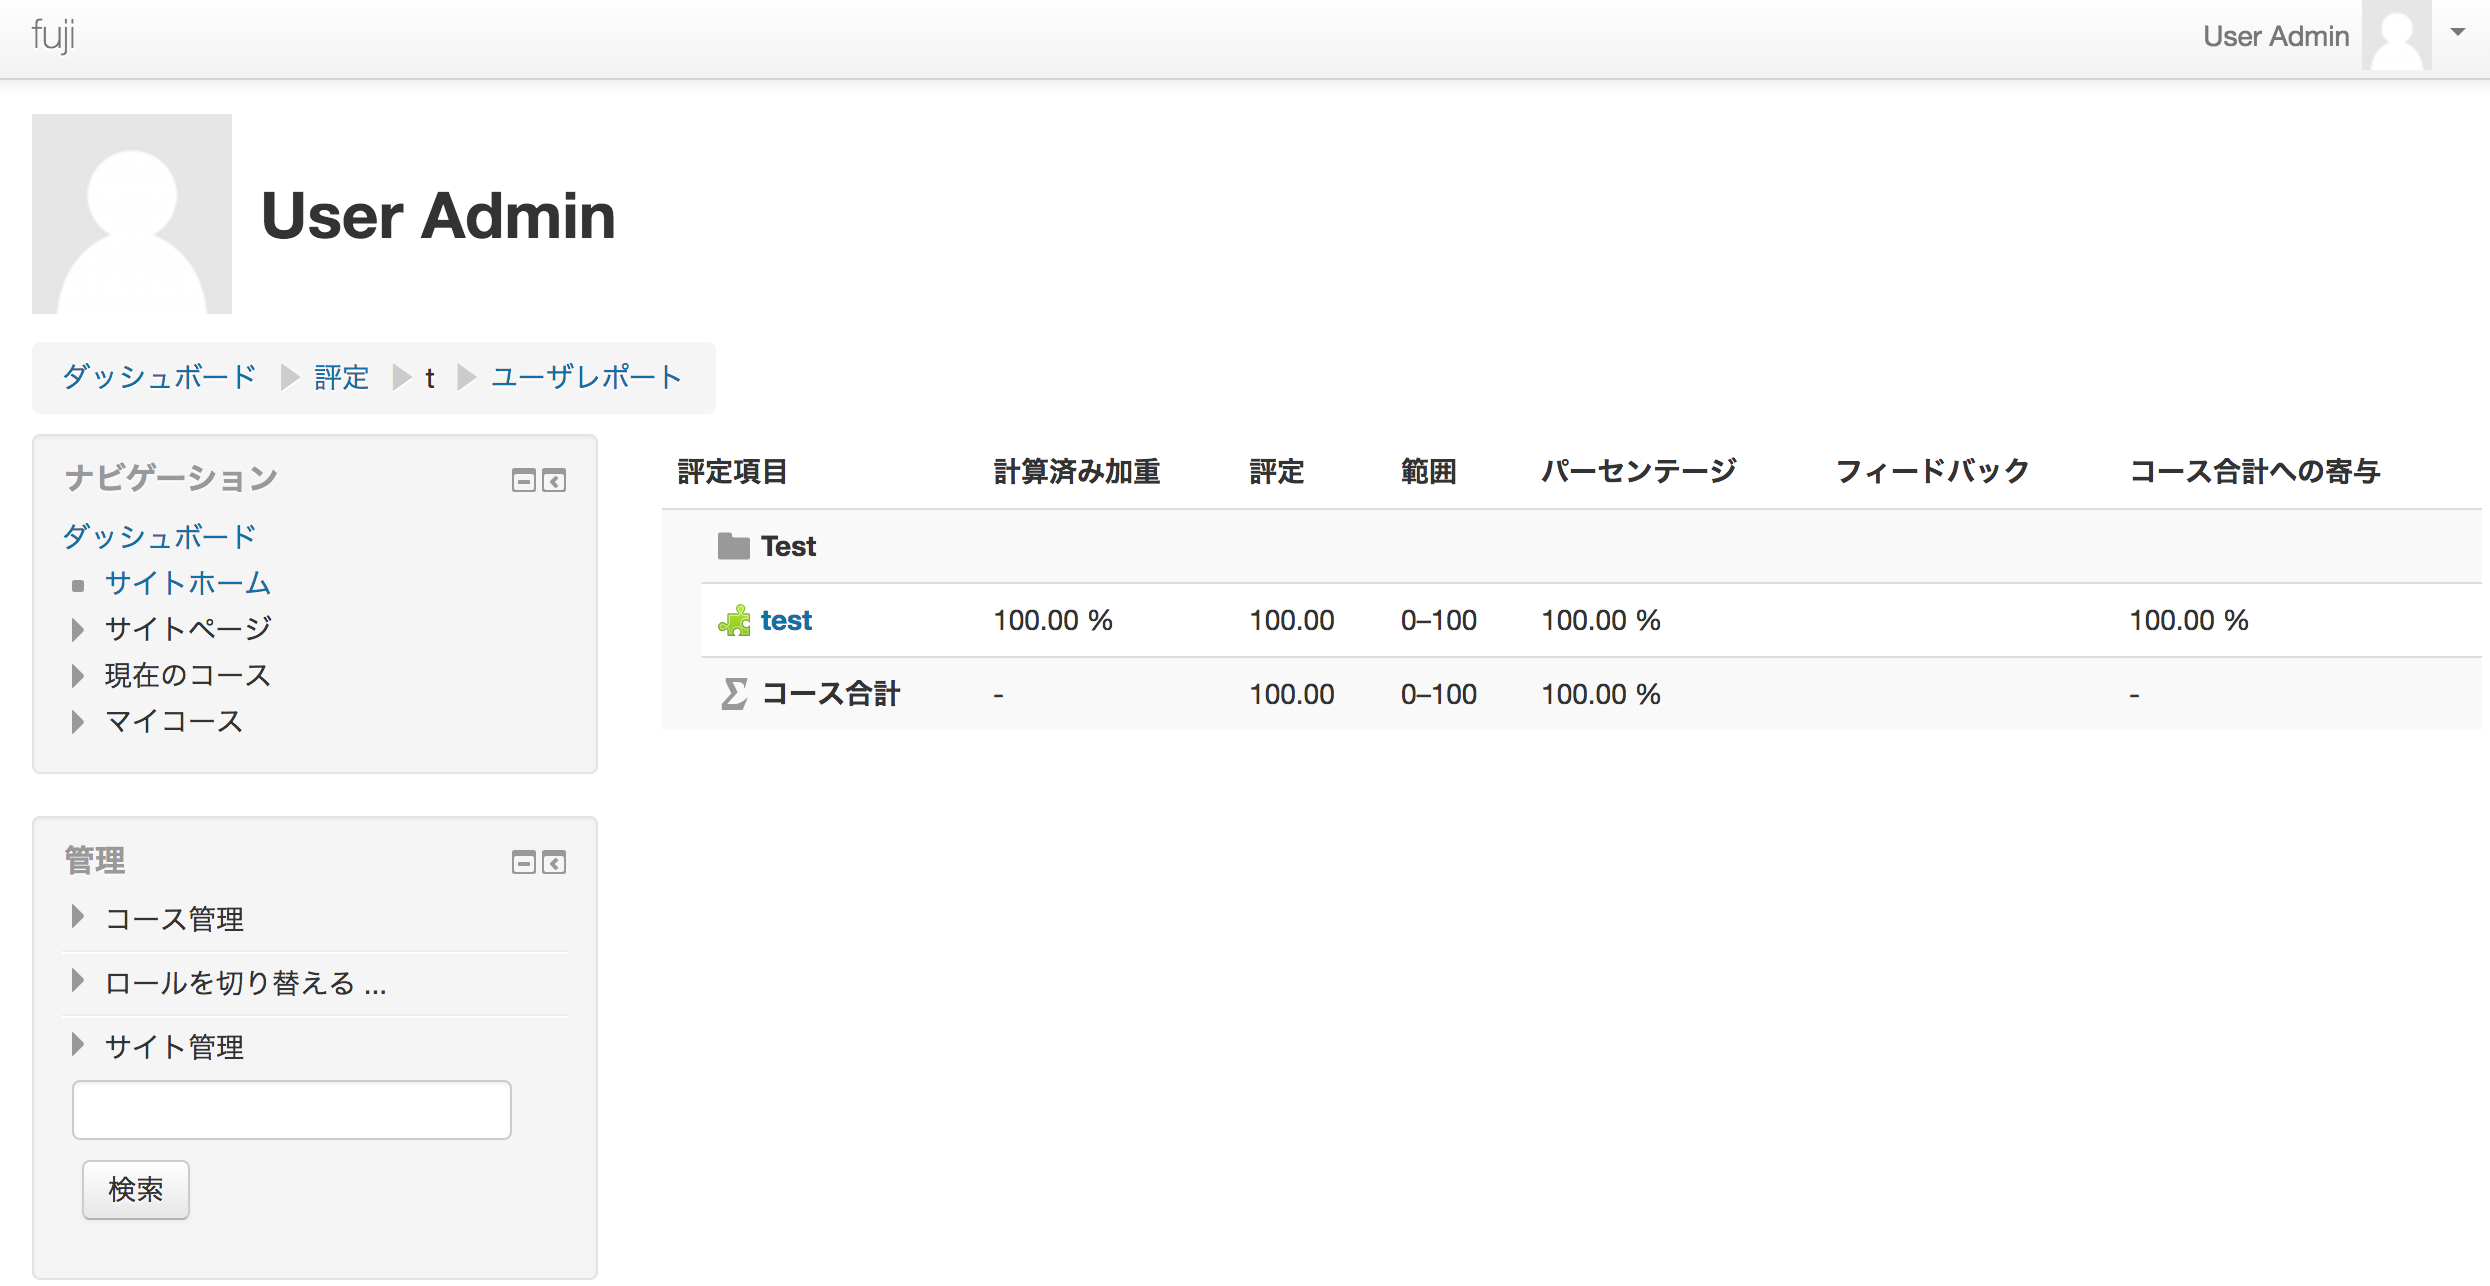
\includegraphics[scale=0.13]{img/score.png}
    \caption{moodle 成績反映}
    \label{fig:moodle score}
  \end{center}
\end{figure}
